%%%%%%%%%%%%%%%%%%%%%%%%%%%%%%%%%%%%%%%
% presentation.tex
%
% This presentation has been designed to install the basics of Git into
% Computer Science students at the University of Hertfordshire.
%
% @author B[]
%%%%%%%%%%%%%%%%%%%%%%%%%%%%%%%%%%%%%%%

\documentclass{beamer}

\usepackage{color}
\usepackage{listings}
\PassOptionsToPackage{hyphens}{url}\usepackage{hyperref}

\usetheme{metropolis}

\definecolor{Blue}{rgb}{0.0, 0.0, 0.8}
\definecolor{DarkGreen}{rgb}{0.0, 0.5, 0.0}
\definecolor{DarkGray}{rgb}{0.5, 0.5, 0.5}
\definecolor{Gray}{rgb}{0.8, 0.8, 0.8}
\definecolor{Orange}{rgb}{0.8, 0.5, 0.0}
\definecolor{White}{rgb}{1.0, 1.0, 1.0}

\lstset{
  basicstyle=\ttfamily\footnotesize,
  breakatwhitespace=false,
  breaklines=true,
  captionpos=b,
  commentstyle=\color{DarkGreen},
  escapeinside={\%*}{*)},
  extendedchars=true,
  frameshape={RYR}{Y}{Y}{RYR},
  keepspaces=true,
  keywordstyle=\color{Blue},
  numbers=left,
  numbersep=6pt,
  numberstyle=\tiny\color{DarkGray},
  rulecolor=\color{Gray},
  showspaces=false,
  showstringspaces=false,
  showtabs=false,
  stepnumber=1,
  stringstyle=\color{Orange},
  tabsize=2
}

\title{Git Basics}
\date{November, 2016}
\author{Daniel Barry}
\institute{University of Hertfordshire}

\begin{document}
  \maketitle
  %%%%%%%%%%%%%%%%%%%%%%%%%%%%%%%%%%%%%%%
  % Introduction
  %%%%%%%%%%%%%%%%%%%%%%%%%%%%%%%%%%%%%%%
  \section{Introduction}
  \begin{frame}{Why use Git?}
    \begin{itemize}
      \item Replace the old ``copy and rename" workflow
      \item History of how the project was built
      \item Ability to go back to any point during the project
      \item Always having a working version
      \item Work in teams easily
      \item Access to large open source projects
      \item Employers prefer you know how repositories work
    \end{itemize}
    This presentation was built in a Git repository!
  \end{frame}
  \begin{frame}{Quick Git History}
    \begin{itemize}
      \item \emph{Patches and Archives} for Linux Kernel (1991 - 2002)
      \item \emph{BitKeeper} for Linux Kernel (2002 - 2005)
      \item In 2005, BitKeeper no longer free (Larry McVoy)
      \item Linus Torvalds designed \emph{Git} to be fast, simple, non-linear,
        distributed and scalable
      \item \emph{Git} for Linux Kernel (2005 - now)
    \end{itemize}
    More:
    \url{https://en.wikipedia.org/wiki/Git}
  \end{frame}
  \begin{frame}{What is Git?}
    \begin{itemize}
      \item Inspired by BitKeeper
      \item Version control system
      \item Fully distributed
      \item Merges, even three-way merges
      \item Robust against corruption
    \end{itemize}
    Git was named after Linus...
  \end{frame}
  \begin{frame}{Branches?}
    \centering
    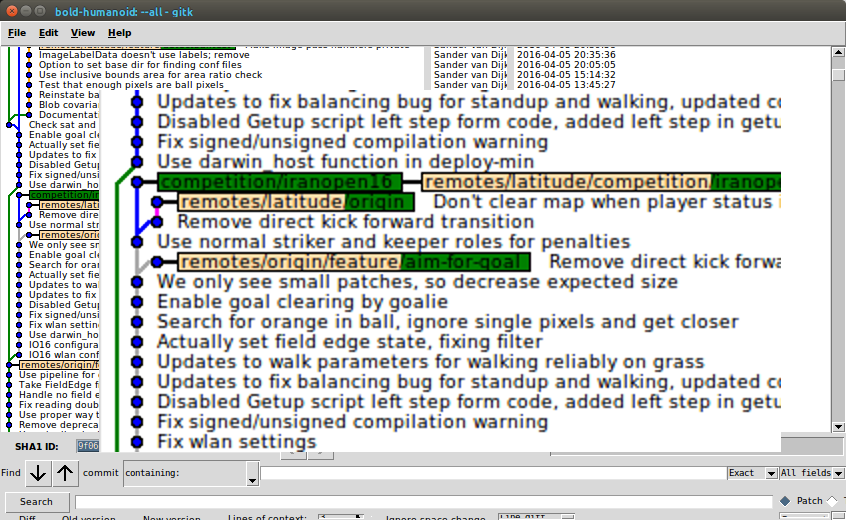
\includegraphics[scale=0.3,keepaspectratio]{gitk-branches.png}
  \end{frame}
  \begin{frame}{What is a Commit?}
    \begin{itemize}
      \item A commit is a series of changes to files
      \item Contains meta information (who, when, etc)
      \item Usually all the changes are related
      \item A small (typically $ \leqslant $ 80 character) message describing
        them
    \end{itemize}
  \end{frame}
  \begin{frame}{What is a Change?}
    \centering
    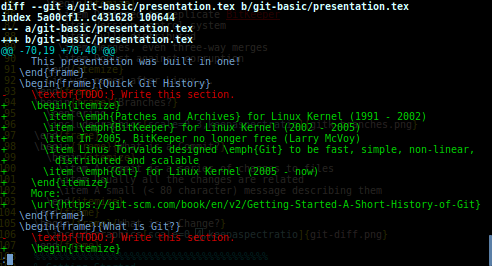
\includegraphics[scale=0.5,keepaspectratio]{git-diff.png}
  \end{frame}
  %%%%%%%%%%%%%%%%%%%%%%%%%%%%%%%%%%%%%%%
  % Getting Started
  %%%%%%%%%%%%%%%%%%%%%%%%%%%%%%%%%%%%%%%
  \section{Getting Started}
  \begin{frame}{Requirements}
    \begin{itemize}
      \item \texttt{git} - The repository program
      \item \texttt{git-gui} - Graphical representation
    \end{itemize}
  \end{frame}
  \begin{frame}[fragile=singleslide]{Setup an Environment}
    Create the working directory and navigate to it
    \begin{lstlisting}[language=bash]
$ mkdir wrk_dir
$ cd wrk_dir
    \end{lstlisting}
    Initialise the repository in the working directory
    \lstinputlisting{out/test1.txt}
  \end{frame}
  %%%%%%%%%%%%%%%%%%%%%%%%%%%%%%%%%%%%%%%
  % Workflow
  %%%%%%%%%%%%%%%%%%%%%%%%%%%%%%%%%%%%%%%
  \section{Workflow}
  \begin{frame}[fragile=singleslide]{Fetching}
    Check for changes from remote repositories
    \lstinputlisting{out/test2.txt}
    This means we must setup a remote
    \lstinputlisting{out/test3.txt}
  \end{frame}
  \begin{frame}[fragile=singleslide]{Status}
    Find out the state of the working tree
    \lstinputlisting{out/test4.txt}
    \begin{itemize}
      \item We are on our master branch
      \item Our latest commit
      \item The fact there is nothing to commit
      \item How to commit if we need to
    \end{itemize}
  \end{frame}
  \begin{frame}[fragile=singleslide]{Adding Files}
    Create simple read me file
    \lstinputlisting{out/test5.txt}
    \lstinputlisting{out/test6.txt}
  \end{frame}
  \begin{frame}[fragile=singleslide]
    Add the file to the commit
    \lstinputlisting{out/test7.txt}
    \lstinputlisting{out/test8.txt}
  \end{frame}
  \begin{frame}{Visually Adding Files}
    \centering
    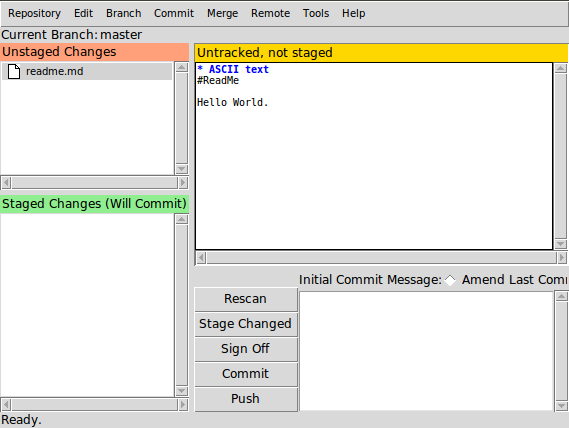
\includegraphics[scale=0.4,keepaspectratio]{git-gui.png}
  \end{frame}
  \begin{frame}[fragile=singleslide]{Commiting \& Pushing}
    Next we commit our changes
    \lstinputlisting{out/test9.txt}
    We fetch to check nothing happened in origin
    \lstinputlisting{out/test10.txt}
  \end{frame}
  \begin{frame}[fragile=singleslide]
    And then we push
    \lstinputlisting{out/test11.txt}
    Now we check our working tree
    \lstinputlisting{out/test12.txt}
  \end{frame}
  \begin{frame}[fragile=singleslide]{Stashing}
    We can create changes and check them
    \lstinputlisting{out/test14.txt}
  \end{frame}
  \begin{frame}[fragile=singleslide]
    Stash our changes
    \lstinputlisting{out/test15.txt}
    Check the status of the repository
    \lstinputlisting{out/test16.txt}
  \end{frame}
  \begin{frame}[fragile=singleslide]
    Pop our changes back
    \lstinputlisting{out/test17.txt}
    We are told the repository status
  \end{frame}
  \begin{frame}[fragile=singleslide]{Pulling}
    Somebody on our team has pushed a change we want
    \lstinputlisting{out/test18.txt}
    Stash our unstaged changes
    \lstinputlisting{out/test19.txt}
  \end{frame}
  \begin{frame}[fragile=singleslide]
    Pull in the changes (auto-rebase)
    \lstinputlisting{out/test20.txt}
  \end{frame}
  \begin{frame}[fragile=singleslide]
    And pop our stashed changes back
    \lstinputlisting{out/test21.txt}
  \end{frame}
  \begin{frame}[fragile=singleslide]{Feature Branch}
    New features developed on a separate branch
    \lstinputlisting{out/test22.txt}
    Check which branch we are on
    \lstinputlisting{out/test23.txt}
  \end{frame}
  \begin{frame}[fragile=singleslide]
    Create change on branch and commit it
    \lstinputlisting{out/test24.txt}
    Push change
    \lstinputlisting{out/test25.txt}
  \end{frame}
  \begin{frame}[fragile=singleslide]{Merge Branch}
    Checkout the master branch
    \lstinputlisting{out/test26.txt}
    Merge the branch with master
    \lstinputlisting{out/test27.txt}
  \end{frame}
  \begin{frame}[fragile=singleslide]
    Now check the status
    \lstinputlisting{out/test28.txt}
    Commits from the branch are waiting to be pushed
  \end{frame}
  %%%%%%%%%%%%%%%%%%%%%%%%%%%%%%%%%%%%%%%
  % Something Went Wrong
  %%%%%%%%%%%%%%%%%%%%%%%%%%%%%%%%%%%%%%%
  \section{Something Went Wrong}
  \begin{frame}[fragile=singleslide]{Undo-ing Changes}
    Check our bad change
    \lstinputlisting{out/test29.txt}
    Undo all changes in file
    \lstinputlisting{out/test30.txt}
  \end{frame}
  \begin{frame}[fragile=singleslide]{Undo-ing Commits}
    Show the previous commit
    \lstinputlisting{out/test31.txt}
    Undo the previous commit
    \lstinputlisting{out/test32.txt}
  \end{frame}
  \begin{frame}[fragile=singleslide]
    Show the previous commit (again)
    \lstinputlisting{out/test33.txt}
    ``Bang, and the dirt is gone!"
  \end{frame}
  \begin{frame}[fragile=singleslide]
    Actually, it is still staged
    \lstinputlisting{out/test34.txt}
    So we can do something with this
  \end{frame}
  %%%%%%%%%%%%%%%%%%%%%%%%%%%%%%%%%%%%%%%
  % Advanced
  %%%%%%%%%%%%%%%%%%%%%%%%%%%%%%%%%%%%%%%
  \section{Advanced}
  \begin{frame}{Re-Writing History}
    \textbf{WARNING:} This is dangerous (but powerful ;) )
    \\
    Reasons not to do this:
    \begin{itemize}
      \item Could make data hard to recover
      \item Will could problems for team mates
      \item More difficult to undo these changes (but not impossible)
    \end{itemize}
    Reasons to do this:
    \begin{itemize}
      \item Something bad happened
      \item ``You're a Git Wizard Harry"
    \end{itemize}
  \end{frame}
  \begin{frame}{Re-Write What?}
    \begin{itemize}
      \item Amend previous commit \texttt{git commit --amend}
      \item Amend many commits \texttt{git rebase -i HEAD~N}
      \item Squashing commits (Use interactive rebase)
      \item Split commits (Use interactive rebase)
      \item Filter-Branch (Scripted re-writing)
    \end{itemize}
    Further reading:
    \url{https://git-scm.com/book/en/v2/Git-Tools-Rewriting-History}
  \end{frame}
  %%%%%%%%%%%%%%%%%%%%%%%%%%%%%%%%%%%%%%%
  % Conclusion
  %%%%%%%%%%%%%%%%%%%%%%%%%%%%%%%%%%%%%%%
  \section{Conclusion}
  \begin{frame}{About Presentation}
    \begin{itemize}
      \item Content - \url{https://github.com/danielbarry/presentations}
      \item Presentation - \url{http://www.latex-project.org}
      \item Theme - \url{https://github.com/matze/mtheme}
    \end{itemize}
  \end{frame}
\end{document}
